\documentclass[12pt]{article}
\usepackage{stata}
\usepackage{graphicx}
\usepackage{geometry}
\usepackage{rotating}
\begin{document}







\author{Jesús Lara Jáuregui}
\title{Problem Set 1}
\maketitle


\section{Problem 1. OLS in MATA}
\subsection{Part 1}
\ Results with myreg1
\begin{stlog}. myreg1 lnwage hieduc exp exp2 
{\smallskip}
b[4,1]
            c1
r1   .08264541
r2   .02523881
r3  -.00037668
r4   1.3094414
{\smallskip}
symmetric V[4,4]
            c1          c2          c3          c4
r1   1.195e-06
r2   1.595e-07   .00001683
r3  -4.035e-09  -3.770e-07   8.579e-09
r4  -.00001749  -.00017676   3.899e-06   .00211062
{\smallskip}
\end{stlog}
\ Results with Stata OlS command
\begin{stlog}. quiet reg lnwage hieduc exp exp2
{\smallskip}
. matrix list e(b)
{\smallskip}
e(b)[1,4]
        hieduc         exp        exp2       _cons
y1   .08264541   .02523881  -.00037668   1.3094414
{\smallskip}
. matrix list e(V)
{\smallskip}
symmetric e(V)[4,4]
            hieduc         exp        exp2       _cons
hieduc   1.195e-06
   exp   1.595e-07   .00001683
  exp2  -4.035e-09  -3.770e-07   8.580e-09
 _cons   -.0000175  -.00017676   3.899e-06   .00211066
{\smallskip}
\end{stlog}
\subsection{Part 2}
\ Results with myreg2
\begin{stlog}. hist(num_awards), title("Number of Awards") color("orange")
(bin=14, start=0, width=.42857143)
{\smallskip}
\end{stlog}
\ Results with Stata's OLS and robust standard errors
\begin{stlog}. 
. matrix list e(b)
{\smallskip}
e(b)[1,4]
        hieduc         exp        exp2       _cons
y1   .08264541   .02523881  -.00037668   1.3094414
{\smallskip}
. matrix list e(V)
{\smallskip}
symmetric e(V)[4,4]
            hieduc         exp        exp2       _cons
hieduc   1.520e-06
   exp   1.712e-07   .00001632
  exp2  -4.045e-09  -3.685e-07   8.451e-09
 _cons  -.00002216  -.00016979   3.771e-06   .00208194
{\smallskip}
. 
\end{stlog}

\section{Problem 2. Poisson using Maximum Likelihood}

If $y_i$ is distributed Poission with mean $exp(X^{'}_i \beta)$, hence the likelihood function for a sample of $N$ observations is given by:

$$ L(\beta)=\prod_{i=1}^{N}\frac{1}{y_{i}!}exp((X^{'}\beta)y_i)exp(-exp(X^{'}\beta))$$


And taking logs we get:

$$lnL(\beta)=\sum_{i}^{N}[-exp(X^{'}\beta)+y_i exp(X^{'}\beta)-ln(y_i !)]$$

Which is the form we use for pur maximum-likelihood estimation
\begin{stlog}. hist(num_awards), title("Number of Awards") color("or
> ange")
(bin=14, start=0, width=.42857143)
{\smallskip}
\end{stlog}
\begin{center}
    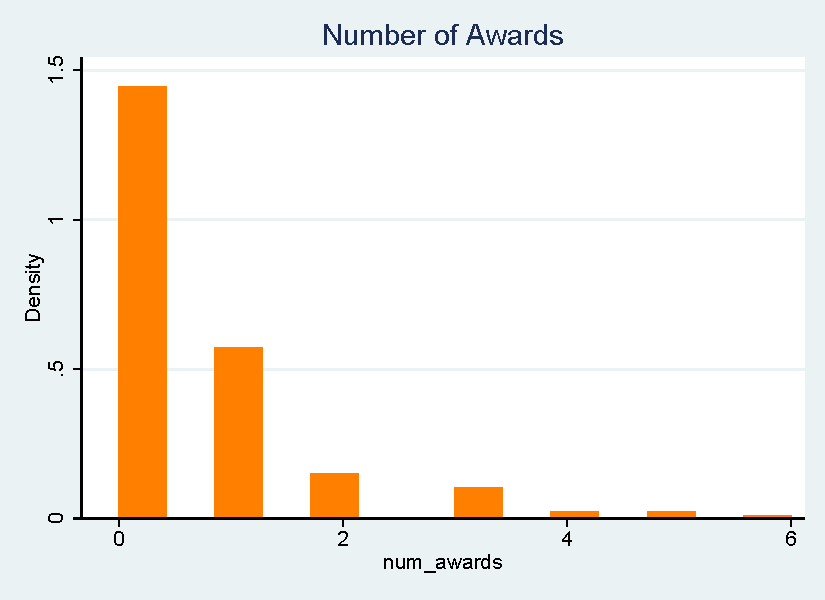
\includegraphics{797B_PS1_JL_5.pdf}
\end{center}
\begin{table}[htbp]\centering
\caption{Number of Awards}
\begin{tabular}{l*{2}{c}}
\toprule
            &        Mean&    Variance\\
\midrule
Number of awards&        0.63&        1.11\\
\bottomrule
\end{tabular}
\end{table}

\begin{table}[htbp]\centering
\def\sym#1{\ifmmode^{#1}\else\(^{#1}\)\fi}
\caption{Poisson Estimation}
\begin{tabular}{l*{2}{c}}
\hline\hline
                &\multicolumn{1}{c}{(1)}&\multicolumn{1}{c}{(2)}\\
                &\multicolumn{1}{c}{Stata Poisson}&\multicolumn{1}{c}{mypois}\\
\hline
main            &                  &                  \\
general         &   0.0000         &   0.0000         \\
                &      (.)         &      (.)         \\
[1em]
academic        &   1.0839\sym{**} &   1.0839\sym{**} \\
                & (0.3583)         & (0.3583)         \\
[1em]
vocation        &   0.3698         &   0.3698         \\
                & (0.4411)         & (0.4411)         \\
[1em]
math score      &   0.0702\sym{***}&   0.0702\sym{***}\\
                & (0.0106)         & (0.0106)         \\
[1em]
Constant        &  -5.2471\sym{***}&  -5.2471\sym{***}\\
                & (0.6585)         & (0.6585)         \\
\hline
Observations    &      200         &      200         \\
\hline\hline
\multicolumn{3}{l}{\footnotesize Standard errors in parentheses}\\
\multicolumn{3}{l}{\footnotesize \sym{*} \(p<0.05\), \sym{**} \(p<0.01\), \sym{***} \(p<0.001\)}\\
\end{tabular}
\end{table}

\section{Problem 3. Mean Squared Error simulation - Sample Size and Distribution}

\begin{table}[htbp]\centering
\caption{Average of the squared error (MSE): OLS and Poisson}
\begin{tabular}{l*{6}{c}}
\toprule
            &    0.01 OLS&   0.01 POIS&     0.1 OLS&    0.1 POIS&       1 OLS&      1 POIS\\
\midrule
N=50        &     .147573&    .0070057&    .1463649&    .0072342&     .143837&    .0077137\\
N=1000      &    .1223382&     .000118&    .1228836&    .0001196&    .1214063&    .0001158\\
\bottomrule
\end{tabular}
\end{table}

\section{Problem 4. Small number of clusters - Wild Bootstrap}
\begin{table}[htbp]\centering
\caption{Coefficient of treatment significant? Frecuency}
\begin{tabular}{l*{2}{c}}
\toprule
            &     Cluster&   Bootstrap\\
\midrule
lnemp       &          10&           0\\
lnemp2      &          10&           1\\
\bottomrule
\end{tabular}
\end{table}

\begin{table}[htbp]\centering
\caption{Coefficient of treatment insignificant? Frecuency}
\begin{tabular}{l*{2}{c}}
\toprule
            &     Cluster&   Bootstrap\\
\midrule
lnemp       &           0&          10\\
lnemp2      &           0&           9\\
\bottomrule
\end{tabular}
\end{table}

\begin{table}[htbp]\centering
\caption{Coefficient of treatment significant? Frecuency (few clusters)}
\begin{tabular}{l*{2}{c}}
\toprule
            &     Cluster&   Bootstrap\\
\midrule
lnemp       &         918&          48\\
lnemp2      &         918&           0\\
\bottomrule
\end{tabular}
\end{table}

\begin{table}[htbp]\centering
\caption{Coefficient of treatment insignificant? Frecuency (few clusters)}
\begin{tabular}{l*{2}{c}}
\toprule
            &     Cluster&   Bootstrap\\
\midrule
lnemp       &           0&          94\\
lnemp2      &           0&          97\\
\bottomrule
\end{tabular}
\end{table}


\end{document}

